
\iffalse
\documentclass[12pt]{article}
\usepackage{graphicx}
\usepackage{amsmath}
\usepackage{mathtools}
\usepackage{gensymb}
\usepackage[latin1]{inputenc}
\usepackage{fullpage}
\usepackage{color}
\usepackage{array}
\usepackage{longtable}
\usepackage{calc}
\usepackage{multirow}
\usepackage{hhline}
\usepackage{ifthen}
\usepackage{booktabs}
\usepackage{graphicx}
\def\inputGnumericTable{}

\newcommand{\mydet}[1]{\ensuremath{\begin{vmatrix}#1\end{vmatrix}}}
\providecommand{\brak}[1]{\ensuremath{\left(#1\right)}}
\providecommand{\norm}[1]{\left\lVert#1\right\rVert}
\newcommand{\solution}{\noindent \textbf{Solution: }}
\newcommand{\myvec}[1]{\ensuremath{\begin{pmatrix}#1\end{pmatrix}}}
\let\vec\mathbf

\begin{document}
\begin{center}
\textbf\large{CHAPTER-9 \\ CIRCLES}

\end{center}
\begin{enumerate}
\section{EXERCISE-10.5}
\section{SOLUTION}
\fi
The input parameters are listed in Table
\ref{tab:chapters/9/10/5/2/}.	
\begin{table}[h!]
	\begin{tabular}{|c|c|p{5cm}|}
\hline
\textbf{Symbol} & \textbf{Value} & \textbf{Description} \\
\hline
$\theta$ & $30\degree$ & $\angle{BAP} = \angle{BAQ}$ \\
\hline
$a$ & $9$ & $AB$ \\
\hline
$c$ & $8$ & $AQ$ \\
\hline
$\vec{e}_1$ & $\myvec{1\\0}$ & Basis vector \\
\hline
\end{tabular}

\caption{}
\label{tab:chapters/9/10/5/2/}	
\end{table}
Take three points Q,R and P on a unit circle  at angles $\theta,\alpha,\text{ and }\beta$. Then
\begin{align}
	\vec{Q} &= \myvec{\cos\theta\\ \sin\theta},\,
	\vec{R} = \myvec{\cos\alpha\\ \sin\alpha},\,
	\vec{S} = \myvec{\cos\beta\\ \sin\beta}
	\\
	\cos\angle QRP&= \frac{\brak{\vec{Q}-\vec{R}}^{\top}\brak{\vec{P}-\vec{R}}}{\norm{\vec{Q}-\vec{R}}\norm{\vec{P}-\vec{R}}}\label{eq:chapters/9/10/5/2/2}
\end{align}
where
\begin{align}
\brak{\vec{Q}-\vec{R}}^{\top}\brak{\vec{P}-\vec{R}}&= \brak{\cos\alpha-\cos\theta}\cos\alpha+\brak{\sin\theta-\sin\alpha}\label{eq:chapters/9/10/5/2/6}
\end{align}
and 
\begin{align}
\norm{\vec{Q}-\vec{R}}^2\norm{\vec{P}-\vec{R}}^2 =\brak{2-2\cos\theta\cos\alpha-2\sin\theta\sin\alpha}\brak{2-\cos\alpha}\label{eq:chapters/9/10/5/2/8}
\end{align}
Substituing \eqref{eq:chapters/9/10/5/2/6} and \eqref{eq:chapters/9/10/5/2/8} in \eqref{eq:chapters/9/10/5/2/2},
\begin{align}
\cos\angle QRP \implies \angle QRP&=62\degree
\end{align}
Similarly, 
\begin{align}
\brak{\vec{Q}-\vec{S}}^{\top}\brak{\vec{P}-\vec{S}}=\brak{\cos\beta-\cos\theta}\cos\beta+\brak{\sin\theta-\sin\beta}\label{eq:chapters/9/10/5/2/16}
\end{align}
and
\begin{align}
\norm{\vec{Q}-\vec{S}}^2\norm{\vec{P}-\vec{S}}^2 =\brak{2-2\cos\theta\cos\beta-2\sin\theta\sin\beta}\brak{2-\cos\beta}\label{eq:chapters/9/10/5/2/18}
\end{align}
Substituing \eqref{eq:chapters/9/10/5/2/16} and \eqref{eq:chapters/9/10/5/2/18} in \eqref{eq:chapters/9/10/5/2/18},
\begin{align}
\cos\angle QSP&=\frac{1.048}{1.098}\\
\implies \angle QSP&=17\degree
\end{align}
See Fig. 
		\ref{fig:chapters/9/10/5/2/Figure}.
\begin{figure}[h]
\centering
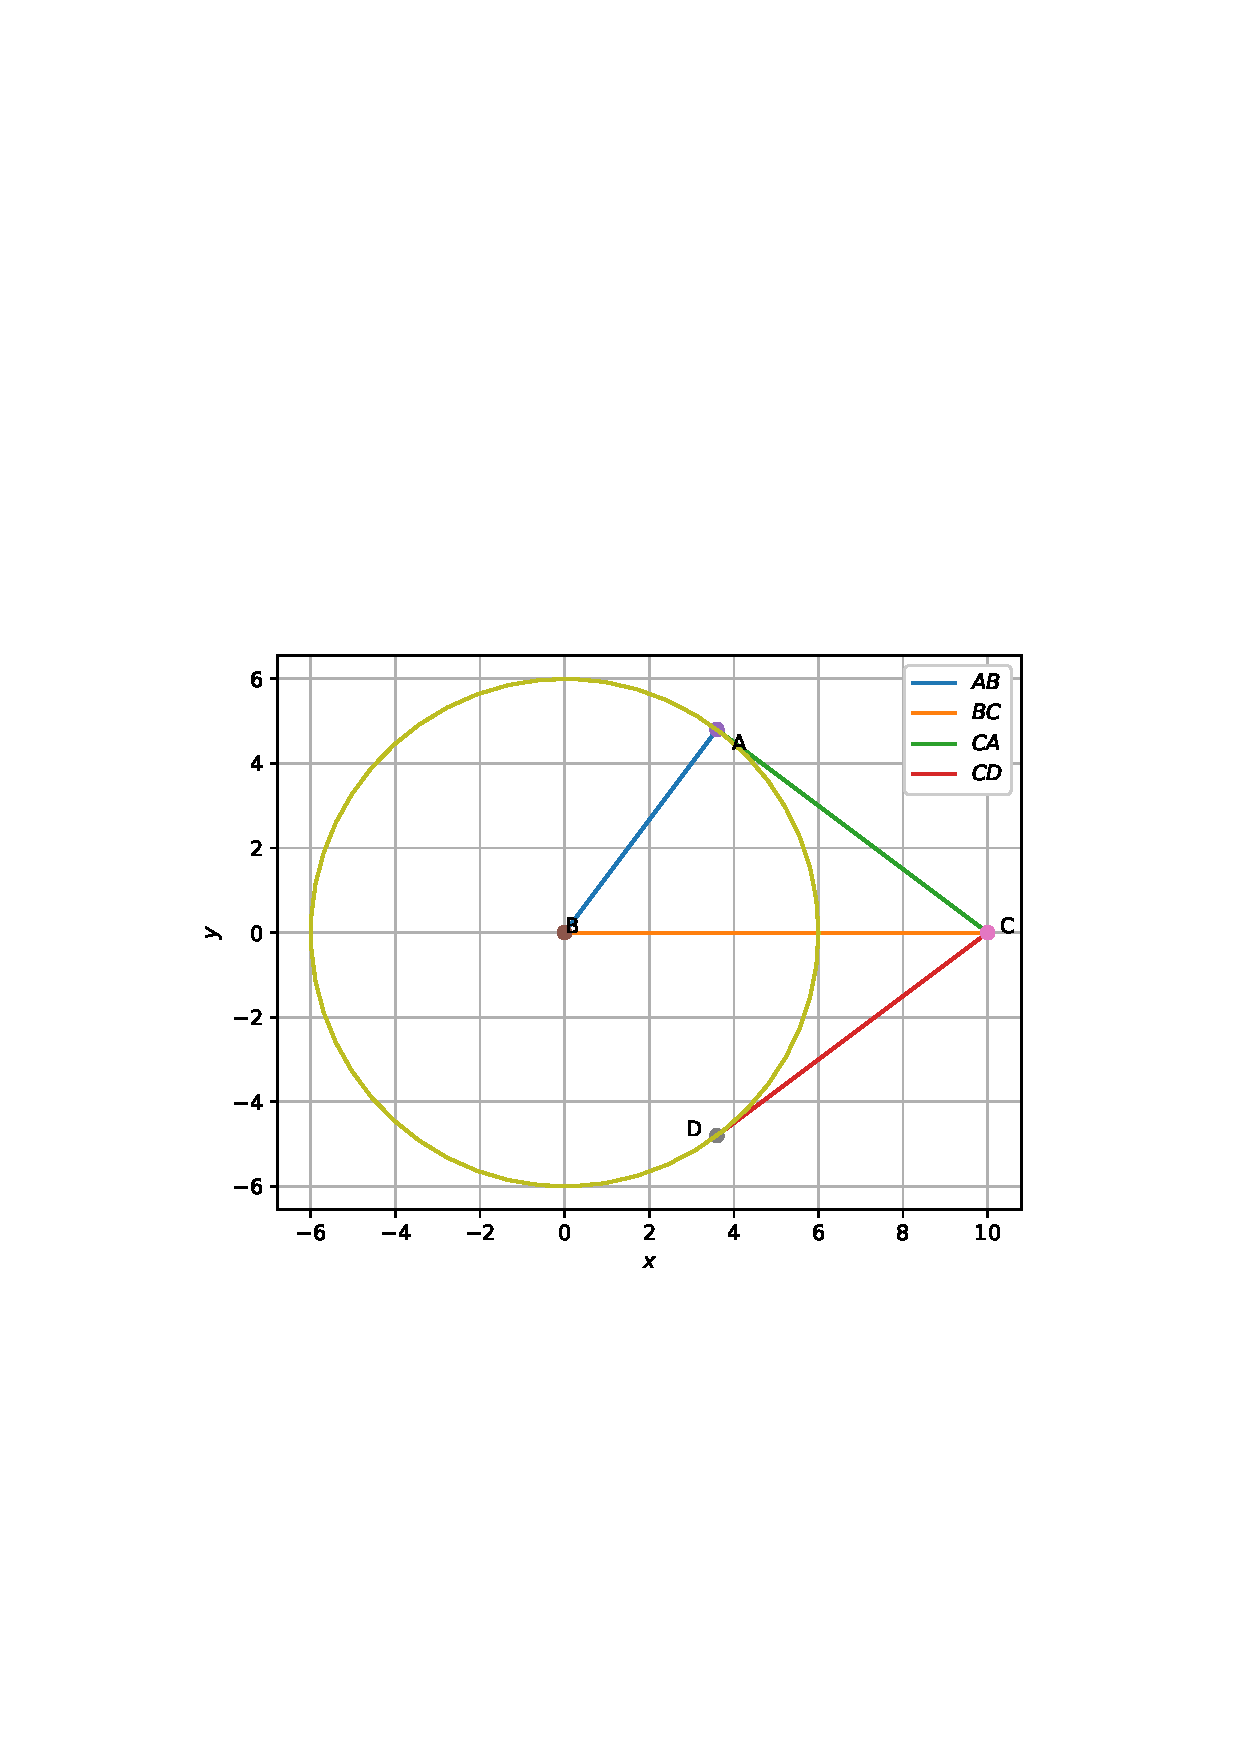
\includegraphics[width=\columnwidth]{chapters/9/10/5/2/figs/circle.png}
\caption{}
		\label{fig:chapters/9/10/5/2/Figure}
\end{figure}
